\section{Use Cases}
\label{sec:use-cases}

\begin{figure}[htb]
	\centering
	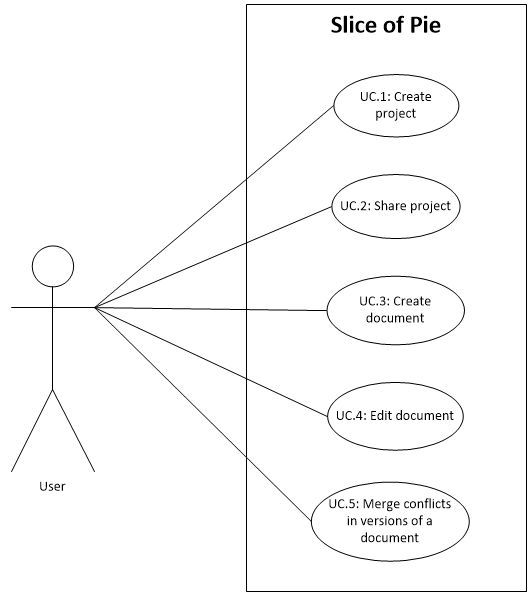
\includegraphics[width=0.7\textwidth]{Appendices/graphics/use-cases-01.png}
	\caption{Use Case diagram of the use cases in SliceOfPie}
	\label{fig:use-cases-01}
\end{figure}

\subsection{UC.1: Create project}
\begin{description}
    \item[Scope] Slice of Pie
    \item[Level] User goal
    \item[Primary actor] User
    \item[Stakeholders and Interests] None
\end{description}
    
\subsubsection{Main Success Scenario}
\begin{enumerate}
    \item User creates a named project
\end{enumerate}
    
\subsubsection{Extensions}
\begin{description}
    \item[UC.1 exA] The user may create projects without a connection to the central storage. In this case the create process is split: The project is created locally, and then synchronized to the central storage later.
\end{description}

\subsection{UC.2: Share project}
\begin{description}
    \item[Scope] Slice of Pie
    \item[Level] User goal
    \item[Primary actor] User
    \item[Stakeholders and Interests] None
\end{description}
    
\subsubsection{Main Success Scenario}
\begin{enumerate}
    \item User chooses a project to share.
    \item User invites other user(s) to the projects.
    \item At some later point in time, the invited user(s) either accepts or declines the invitation.
\end{enumerate}

\subsection{UC.3: Create folder}
\begin{description}
    \item[Scope] Slice of Pie
    \item[Level] User goal.
    \item[Primary actor] User
    \item[Stakeholders and Interests] None
\end{description}
    
\subsubsection{Main Success Scenario}
\begin{enumerate}
    \item User navigates to a project or folder.
    \item User chooses a name for the folder.
    \item User creates the folder.
    \item The system makes sure the folder is made available to all project participants.
\end{enumerate}
    
\subsubsection{Extensions}
\begin{description}
    \item[UC.3 exA] The user may create folder without a connection to the central storage.
        In this case, the create process is split: The folder is created locally, and then synchronized
        to the central storage later.
\end{description}

\subsection{UC.4: Create document}
\begin{description}
    \item[Scope] Slice of Pie
    \item[Level] User goal.
    \item[Primary actor] User
    \item[Stakeholders and Interests] None
\end{description}
    
\subsubsection{Main Success Scenario}
\begin{enumerate}
    \item User navigates to a project or folder.
    \item User chooses a name for a document.
    \item User creates the document.
    \item The system makes sure the document is made available to all project participants.
\end{enumerate}
    
\subsubsection{Extensions}
\begin{description}
    \item[UC.4 exA] The user may create documents without a connection to the central storage.
        In this case, the create process is split: The document is created locally, and then
        synchronized to the central storage later.
\end{description}

\subsection{UC.5: Edit document}
\begin{description}
    \item[Scope] Slice of Pie
    \item[Level] Use goal
    \item[Primary actor] User
    \item[Stakeholders and Interests] None
\end{description}

\subsubsection{Main Success Scenario}
\begin{enumerate}
    \item Open an existing document
    \item Edit the document using either the offline or web-based Slice of Pie editor
    \item Save the document
\end{enumerate}
    
\subsubsection{Extensions}
\begin{description}
    \item[UC.5 exA] Instead of opening an existing document, the user may choose to edit a document subsequent to creating it.
    \item[UC.5 exB] The user may edit documents without a connection to the central storage. In this case the save process is split: The document is saved locally, and then synchronized to the central storage later.
\end{description}

\subsection{UC.6: Synchronize project}
\begin{description}
    \item[Scope] Slice of Pie
    \item[Level] User goal
    \item[Primary actor] User
    \item[Stakeholder and interests] None
\end{description}
    
\subsubsection{Main Succes Scenario}
\begin{enumerate}
    \item User chooses a project to synchronize.
    \item Remote changes are downloaded and local changes are uploaded.
\end{enumerate}
    
\subsubsection{Extensions}
\begin{description}
    \item[UC.6 exA] If conflicts occur the GUI will notify the user and user will have the opportunity to resolve conflicts. (See UC.7)
\end{description}
    
\subsection{UC.7: Merge conflicting versions of a document}
\begin{description}
    \item[Scope] Slice of Pie
    \item[Level] User goal
    \item[Primary actor] User
    \item[Stakeholders and Interests] None
\end{description}
    
\subsubsection{Main Success Scenario}
\begin{enumerate}
    \item One or more users have edited the document offline, resulting in a conflict between two versions.
    \item The last user to synchronize with central storage will be presented with a merged version of the two conflicting documents, and will have the option to edit it before accepting it as the final version. Alternatively, the user can choose to keep either the present or his own version, discarding the other.
\end{enumerate}